\section{experimentation/simulation/testing/results}
%%%%%%%%%%%%%%%%%%%%%%%%%%%%%%%%%%%%%%%%%%%%%%%%%%%%%%%%%%%%%%%%%%%%%%%%%%%%%%%%
%%%%%%%%%%%%%%%%%%%%%%%%%%%%%%%%%%%%%%%%%%%%%%%%%%%%%%%%%%%%%%%%%%%%%%%%%%%%%%%%
%%%%%%%%%%%%%%%%%%%%%%%%%%%%%%%%%%%%%%%%%%%%%%%%%%%%%%%%%%%%%%%%%%%%%%%%%%%%%%%%
\subsection{Experimentation}
%%%%%%%%%%%%%%%%%%%%%%%%%%%%%%%%%%%%%%%%%%%%%%%%%%%%%%%%%%%%%%%%%%%%%%%%%%%%%%%%
%%%%%%%%%%%%%%%%%%%%%%%%%%%%%%%%%%%%%%%%%%%%%%%%%%%%%%%%%%%%%%%%%%%%%%%%%%%%%%%%
%%%%%%%%%%%%%%%%%%%%%%%%%%%%%%%%%%%%%%%%%%%%%%%%%%%%%%%%%%%%%%%%%%%%%%%%%%%%%%%%
\subsection{Simulation}
Simulations performed on system specified by parameters in Tables~\ref{tab:cuk_values} and~\ref{tab:system_values}.
%%%%%%%%%%%%%%%%%%%%%%%%%%%%%%%%%%%%%%%%%%%%%%%%%%%%%%%%%%%%%%%%%%%%%%%%%%%%%%%%
%%%%%%%%%%%%%%%%%%%%%%%%%%%%%%%%%%%%%%%%%%%%%%%%%%%%%%%%%%%%%%%%%%%%%%%%%%%%%%%%
\subsubsection{Specifications}\label{sec:simulation_specifications}
State-space description of system (continuous time)
\begin{align*}
\boldsymbol{A}
&=
\begin{bmatrix}
\texttt{0} & \texttt{0} & \texttt{+4.166667E+04} & \texttt{-4.166667E+04}\\
\texttt{0} & \texttt{-1.218537E+03} & \texttt{0} & \texttt{+1.218537E+05}\\
\texttt{-1.063830E+03} & \texttt{0} & \texttt{-1.816915E+03} & \texttt{-1.421277E+03}\\
\texttt{-1.063830E+03} & \texttt{-2.125959E+03} & \texttt{-1.421277E+03} & \texttt{-1.195715E+03}
\end{bmatrix}
\\[11pt]
\boldsymbol{b}
&=
\begin{bmatrix}
\texttt{0} & \texttt{0} & \texttt{0} & \texttt{0}\\
\texttt{0} & \texttt{0} & \texttt{0} & \texttt{0}\\
\texttt{+2.127660E+03} & \texttt{-1.063830E+03} & \texttt{0} & \texttt{0}\\
\texttt{0} & \texttt{-1.063830E+03} & \texttt{0} & \texttt{0}
\end{bmatrix}
\\[11pt]
\boldsymbol{c}
&=
\begin{bmatrix}
\texttt{0} & \texttt{+9.992006E-01} & \texttt{0} & \texttt{+7.993605E-02}
\end{bmatrix}
\\[11pt]
\boldsymbol{b}_d
&=
\begin{bmatrix}
\texttt{+8.364441E+03}\\
\texttt{0}\\
\texttt{+2.132688E+04}\\
\texttt{-2.034445E+04}
\end{bmatrix}
\end{align*}
%%%%%%%%%%%%%%%%%%%%%%%%%%%%%%%%%%%%%%%%%%%%%%%%%%%%%%%%%%%%%%%%%%%%%%%%%%%%%%%%
Note that this system is controllable from $\hat{d}$, which for a $n$-state system may be checked using the \textsf{MATLAB} call of~(\ref{matlab:controllable})\footnote{Where \texttt{bD} respresents the matrix describing how the control signal enters the system under investigation.} for our 4 state system. There are thus no uncontrollable states and thus $(\boldsymbol{A}, \, \boldsymbol{B})$ is stabilizable from $\hat{d}$ (a condition required to employ LQR control design).
\begin{align}\label{matlab:controllable}
\texttt{rank(ctrb(A, bD)) == n}
\end{align}
% ~\rule{\textwidth}{0.5pt}
%%%%%%%%%%%%%%%%%%%%%%%%%%%%%%%%%%%%%%%%%%%%%%%%%%%%%%%%%%%%%%%%%%%%%%%%%%%%%%%%
State-space description of system (discrete time)
\begin{align*}
\overline{\squarey{\boldsymbol{A} - \boldsymbol{L}\boldsymbol{c}}}
&=
\begin{bmatrix}
\texttt{+5.899444E-04} & \texttt{-6.010730E-02} & \texttt{+5.768492E-04} & \texttt{+6.223055E-02}\\
\texttt{+1.155143E-06} & \texttt{-1.070972E-04} & \texttt{+1.115969E-06} & \texttt{+1.171403E-04}\\
\texttt{-1.052231E-03} & \texttt{+1.040045E-01} & \texttt{-1.024871E-03} & \texttt{-1.095839E-01}\\
\texttt{+5.326313E-06} & \texttt{-5.042553E-04} & \texttt{+5.159615E-06} & \texttt{+5.448561E-04}
\end{bmatrix}
\\[11pt]
\overline{\boldsymbol{b}}
&=
\begin{bmatrix}
\texttt{+3.806479E-02} & \texttt{-9.994101E-01} & \texttt{0} & \texttt{0}\\
\texttt{-1.942447E-05} & \texttt{+1.155143E-06} & \texttt{0} & \texttt{0}\\
\texttt{-9.973269E-03} & \texttt{-1.052231E-03} & \texttt{0} & \texttt{0}\\
\texttt{-1.151095E-04} & \texttt{+5.326313E-06} & \texttt{0} & \texttt{0}
\end{bmatrix}
\\[11pt]
\overline{\boldsymbol{c}}
&=
\begin{bmatrix}
\texttt{0} & \texttt{+9.992006E-01} & \texttt{0} & \texttt{+7.993605E-02}
\end{bmatrix}
\\[11pt]
\overline{\boldsymbol{b}_d}
&=
\begin{bmatrix}
\texttt{-1.809741E+01}\\
\texttt{-3.591587E-04}\\
\texttt{-4.164968E-01}\\
\texttt{-2.157311E-03}
\end{bmatrix}
\end{align*}
\rule{\textwidth}{0.5pt}
LQR - \hl{TODO describe process of determining these weights}
\begin{itemize}
    \item \texttt{w = 1}
    \item \texttt{q = diag([0 0 0 0 100])}
    \item \texttt{r = 1}
\end{itemize}
returns
\begin{itemize}
    \item \texttt{Kf = [+9.671365E-05 +5.727858E-05 +4.957778E-03 -4.808127E-03]}
    \item \texttt{Ki = -10.000000}
\end{itemize}
\rule{\textwidth}{0.5pt}
Observer
\begin{itemize}
    \item \texttt{p = -1.416057E+05}
    \item \texttt{L = [+9.671365E-05 +5.727858E-05 +4.957778E-03 -4.808127E-03]}
    \item \texttt{L\_bar = [-1.924405E+00, +1.000089E+00, -1.049633E-01, +1.039485E-02]}
\end{itemize}
Note that this observer system produces stable $\overline{\squarey{\boldsymbol{A} - \boldsymbol{L}\boldsymbol{c}}}$ (one of the requirements for the observer to generate estimates of state variables such that the error between estimated and actual decays exponentially).
%%%%%%%%%%%%%%%%%%%%%%%%%%%%%%%%%%%%%%%%%%%%%%%%%%%%%%%%%%%%%%%%%%%%%%%%%%%%%%%%
%%%%%%%%%%%%%%%%%%%%%%%%%%%%%%%%%%%%%%%%%%%%%%%%%%%%%%%%%%%%%%%%%%%%%%%%%%%%%%%%
% \subsubsection{Method}
% Notes:
% \begin{itemize}
%     \item ADC conversions and ZOH-discretisation simulated through \textsf{Simulink}'s ZOH blocks
% \end{itemize}
%%%%%%%%%%%%%%%%%%%%%%%%%%%%%%%%%%%%%%%%%%%%%%%%%%%%%%%%%%%%%%%%%%%%%%%%%%%%%%%%
%%%%%%%%%%%%%%%%%%%%%%%%%%%%%%%%%%%%%%%%%%%%%%%%%%%%%%%%%%%%%%%%%%%%%%%%%%%%%%%%
\subsubsection{\textsf{Simulink}}
\begin{figure}[H]
    \centering
    \fbox{
    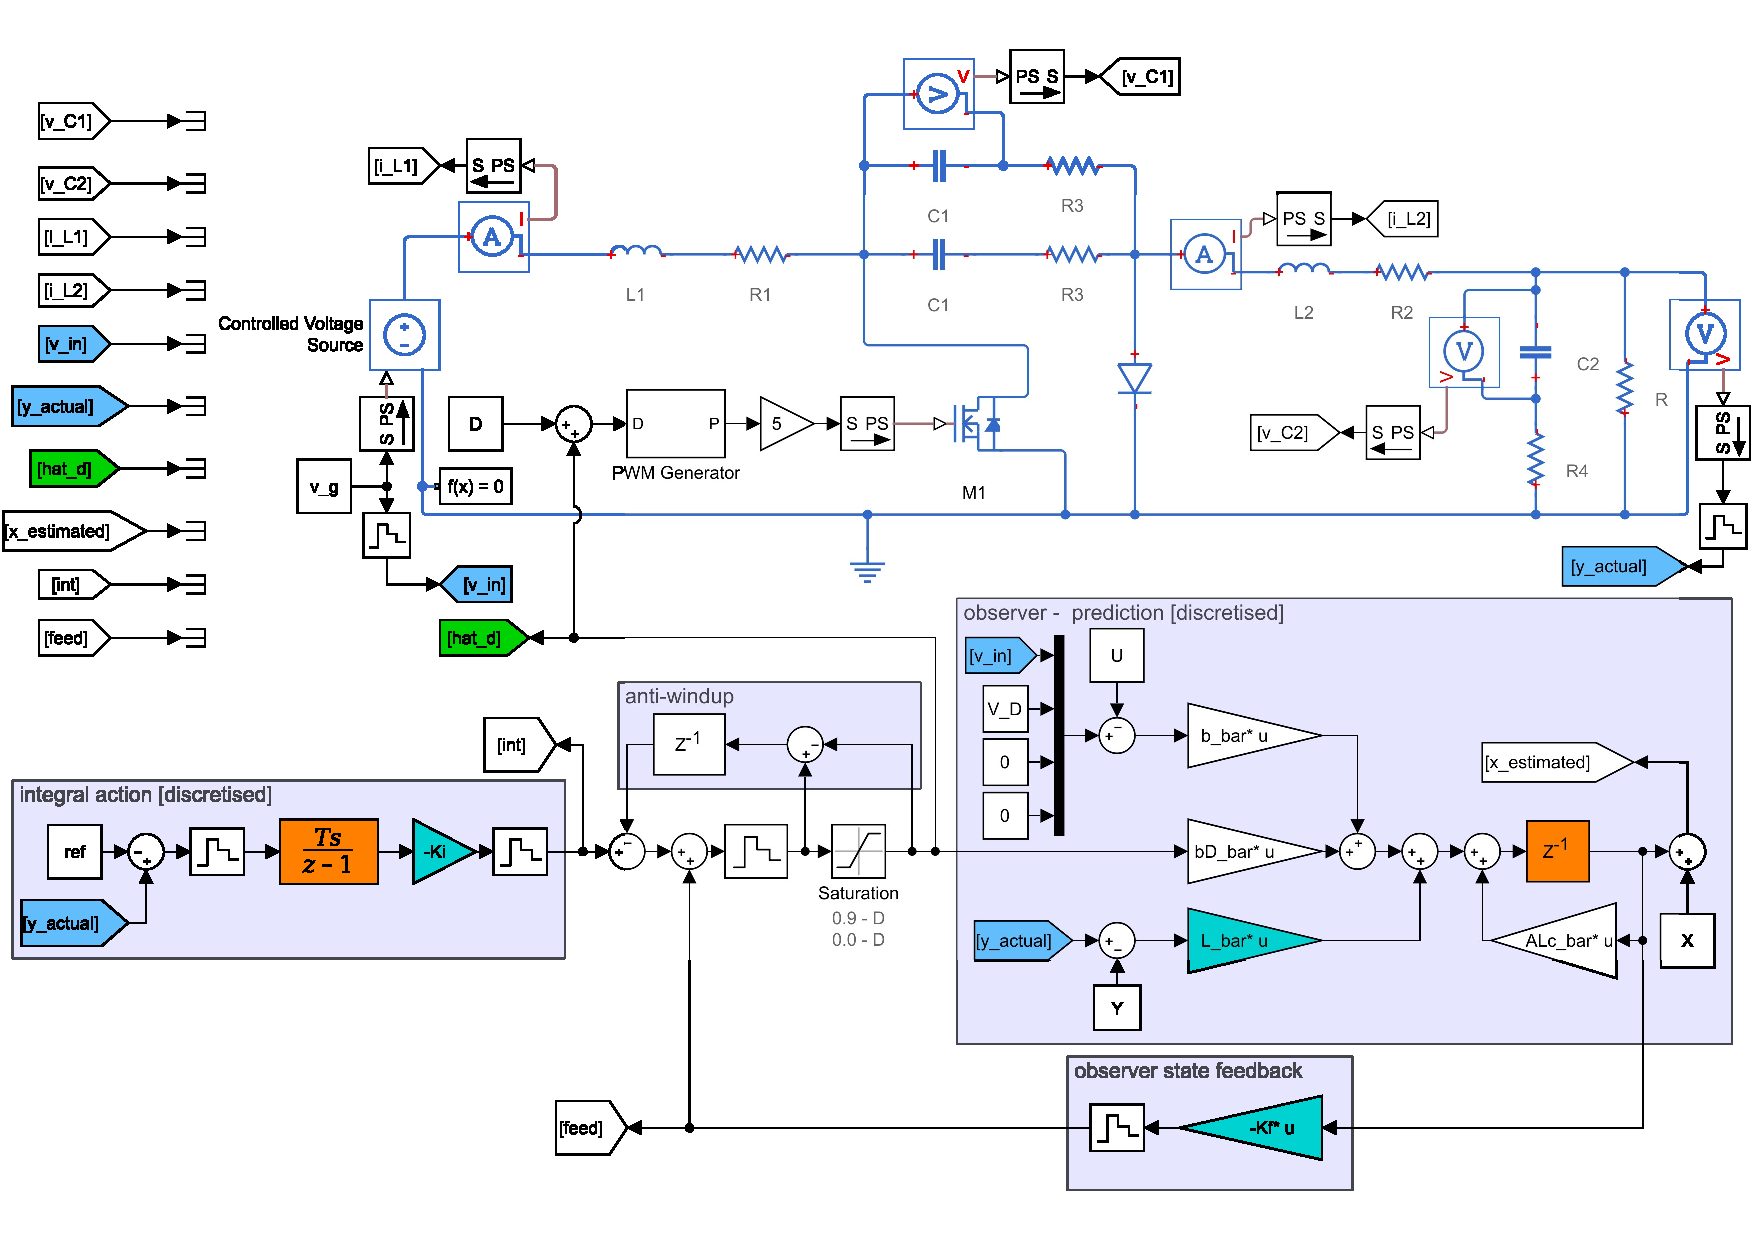
\includegraphics[width = 0.92\textwidth]{figures/simulink.pdf}
    }
    \caption{Simplified \textsf{Simulink} model used to simulate the \'{C}uk converter under augmented control regime of Section~\ref{sec:control_ultimate}}
    \label{fig:simulink}
\end{figure}
Notes:
\begin{itemize}
    \item PWM generator set to switching frequency $f_\text{switching} = 100 \ \mathsf{kHz}$
    \item ZOH blocks configured for sample time \texttt{Ts = 100e-6}
    \item \texttt{ALc\_bar} denotes the matrix $\overline{\squarey{\boldsymbol{A} - \boldsymbol{L}\boldsymbol{c}}}$
\end{itemize}
%%%%%%%%%%%%%%%%%%%%%%%%%%%%%%%%%%%%%%%%%%%%%%%%%%%%%%%%%%%%%%%%%%%%%%%%%%%%%%%%
\begin{figure}[H]
    \centering
    \fbox{
    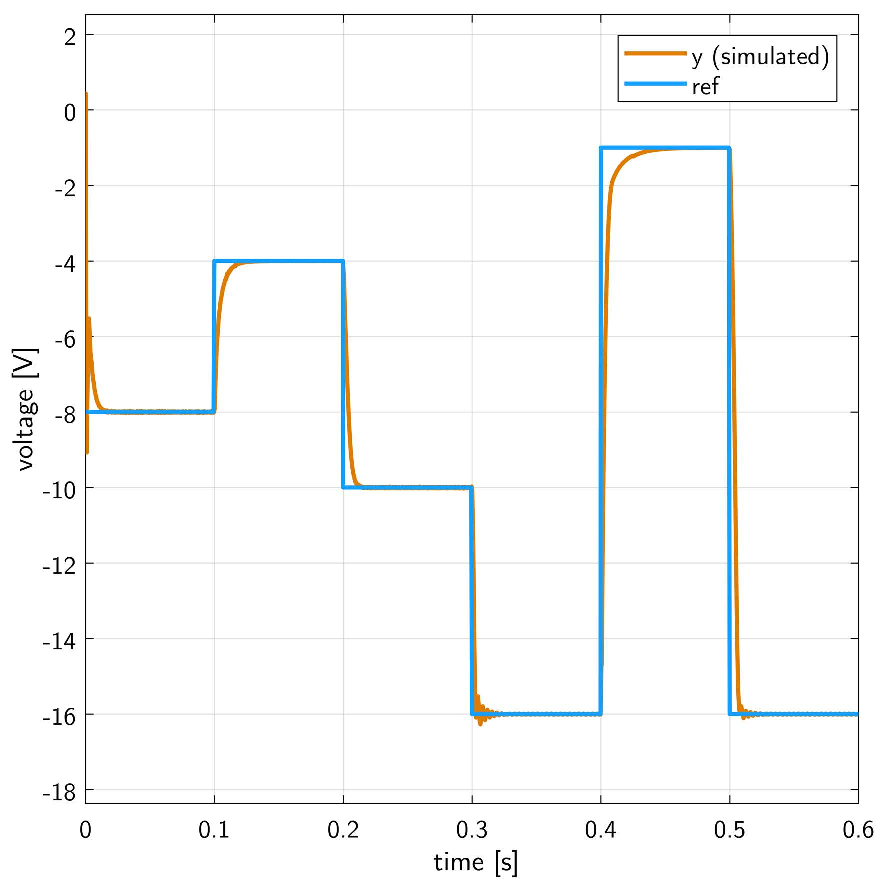
\includegraphics[height = 0.4\textheight]
    {figures/estimation/ref_y_pulsetrain.pdf}
    }
    \caption{Simulated system response to step changes in reference}
    \label{fig:simulation_pulsetrain}
\end{figure}
Some quantities of note from this simulation are provided in Table~\ref{tab:simulation_step}. Quantities maximum unless specified otherwise.
\begin{table}[H]
    \centering
    \begin{tabular}{|c|c|c|c|}
    \hline
    Quantity & Value [S.I.] & Value [\%] & Notes\\
    \hline
    Overshoot & $190 \ \mathsf{mV}$ & $1.2$ & at $\textsf{ref: } \minus 10 \rightarrow \minus 16 \ \mathsf{V}$\\
    \hline
    Output voltage ripple (boost mode) & $21 \ \mathsf{mV}$ & $0.13$ & at $\textsf{ref } = \minus 16 \ \mathsf{V}$\\
    \hline
    Output voltage ripple (buck mode) & $5.4 \ \mathsf{mV}$ & $0.14$ & at $\textsf{ref } = \minus 1 \ \mathsf{V}$\\
    \hline
    Steady-state error & $0$ & $0$ & for these steps $100 \ \mathsf{ms}$ apart\\
    \hline
    \end{tabular}
    \caption{}
    \label{tab:simulation_step}
\end{table}
Additional notes:
\begin{itemize}
    \item transient behaviour upon system turn on discounted in populating Table~\ref{tab:simulation_step}
    \item settling time maximum for reference undergoing step change from greater to lesser magnitude
    \item output takes $\approx 100 \ \mathsf{ms}$ to settle for $\textsf{ref: } \minus 16 \rightarrow \minus 1 \ \mathsf{V}$
\end{itemize}
%%%%%%%%%%%%%%%%%%%%%%%%%%%%%%%%%%%%%%%%%%%%%%%%%%%%%%%%%%%%%%%%%%%%%%%%%%%%%%%%
\begin{figure}[H]
    \centering
    \fbox{
    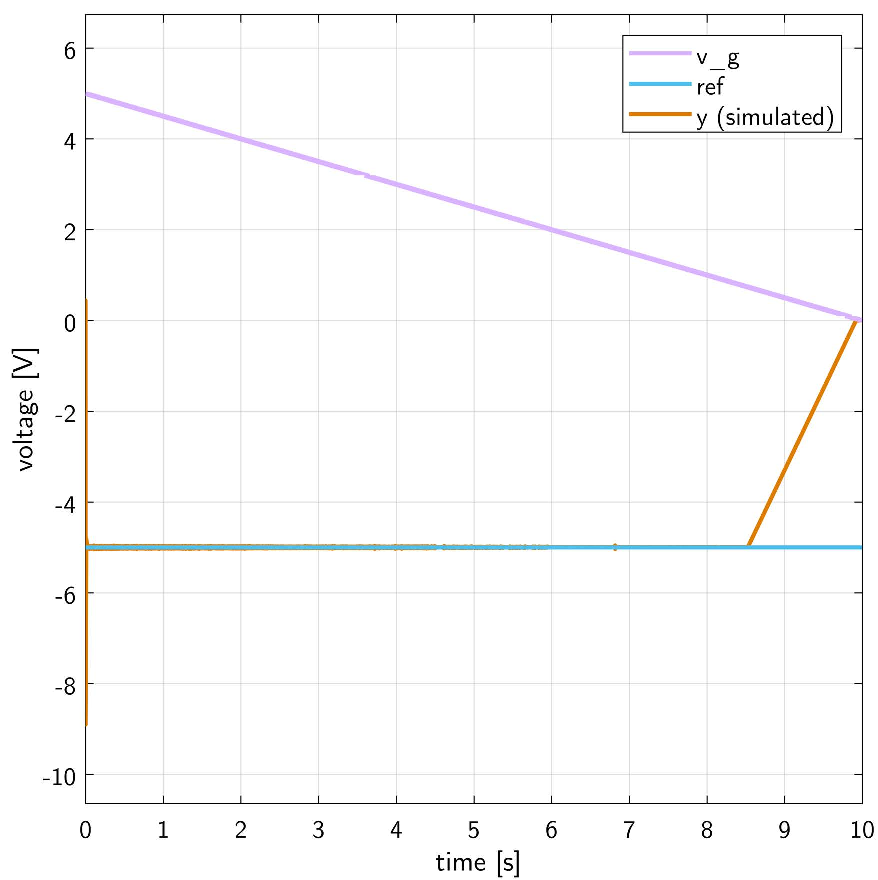
\includegraphics[height = 0.4\textheight]
    {figures/estimation/ref_y_ramp.pdf}
    }
    \caption{Simulated system response to ramp disturbance in input voltage at fixed reference}
    \label{fig:simulation_ramp}
\end{figure}
Some quantities of note from this simulation are provided in Table~\ref{tab:simulation_ramp}. Quantities maximum unless specified otherwise.
\begin{table}[H]
    \centering
    \begin{tabular}{|c|c|c|c|}
    \hline
    Quantity & Value [S.I.] & Value [\%] & Notes\\
    \hline
    Output voltage ripple & $71 \ \mathsf{mV}$ & $1.4$ & Decreases as $v_g$ decreases\\
    \hline
    Steady-state error & $9 \ \mathsf{mV}$ & $0.18$ & Increases rapidly as $v_g$ drops below $0.8 \ \mathsf{V}$\\
    \hline
    \end{tabular}
    \caption{}
    \label{tab:simulation_ramp}
\end{table}
Additional notes:
\begin{itemize}
    \item transient behaviour upon system turn on discounted in populating Table~\ref{tab:simulation_ramp}
    \item $\textsf{ref } = \minus 5 \ \mathsf{V}$ $\implies$ duty ratio saturates at $90 \ \mathsf{\%}$ for $v_g < 0.8 \ \mathsf{V}$
\end{itemize}
%%%%%%%%%%%%%%%%%%%%%%%%%%%%%%%%%%%%%%%%%%%%%%%%%%%%%%%%%%%%%%%%%%%%%%%%%%%%%%%%
%%%%%%%%%%%%%%%%%%%%%%%%%%%%%%%%%%%%%%%%%%%%%%%%%%%%%%%%%%%%%%%%%%%%%%%%%%%%%%%%
%%%%%%%%%%%%%%%%%%%%%%%%%%%%%%%%%%%%%%%%%%%%%%%%%%%%%%%%%%%%%%%%%%%%%%%%%%%%%%%%
\subsection{Testing}
Testing revealed that the gate driver IC did not function as anticipated. It was decided to bypass this IC and drive the \'{C}uk converter MOSFET directly from the microcontroller. This was the configuration used in testing performance of converter circuit powered from microcontroller PWM module.
%%%%%%%%%%%%%%%%%%%%%%%%%%%%%%%%%%%%%%%%%%%%%%%%%%%%%%%%%%%%%%%%%%%%%%%%%%%%%%%%
\subsubsection{Open-loop - characterising transient response}
Testing on \'{C}uk converter begun was observing the transient response at three operation points with $100 \ \mathsf{\Omega}$ resistor as load. The results are provided in Table~\ref{tab:trans}. Simulated output extracted from \textsf{MATLAB} script of Appendix~\ref{apx:MATLAB}. \hl{Note that this test was performed without the gate driver IC connected correctly (and so current to switch converter circuit MOSFET came from microcontroller which was unable to supply that which was required). Upon correct connection of the gate driver IC the difference between output voltages in simulation and hardware was less than $1 \ \mathsf{\%}$.}
\begin{table}[H]
\centering
\begin{tabular}{|c|c|c||c|}
\hline
Duty cycle  & Output voltage & Ripple  & Simulated output \\ \hline \hline
12.5\%      & -925mV         & 52mV     & -975mV \\ \hline
50\%        & -4.5V          & 68mV     & -5.02V\\\hline
62.5 \%     & -12.8V         & 63mV     & -8.38V\\ \hline
\end{tabular}
\caption{Transient response}
\label{tab:trans}
\end{table}
Worst case settling time was found to be $\approx 10 \ \mathsf{ms}$ and was produced for $y \text{: } \minus 0.925 \rightarrow \minus 12.8 \ \mathsf{V}$. \hl{TODO explain right arrow notation}
%%%%%%%%%%%%%%%%%%%%%%%%%%%%%%%%%%%%%%%%%%%%%%%%%%%%%%%%%%%%%%%%%%%%%%%%%%%%%%%%
\subsubsection{Open-loop - mapping duty ratio to output voltage}
\begin{figure}[H]
\centering
\fbox{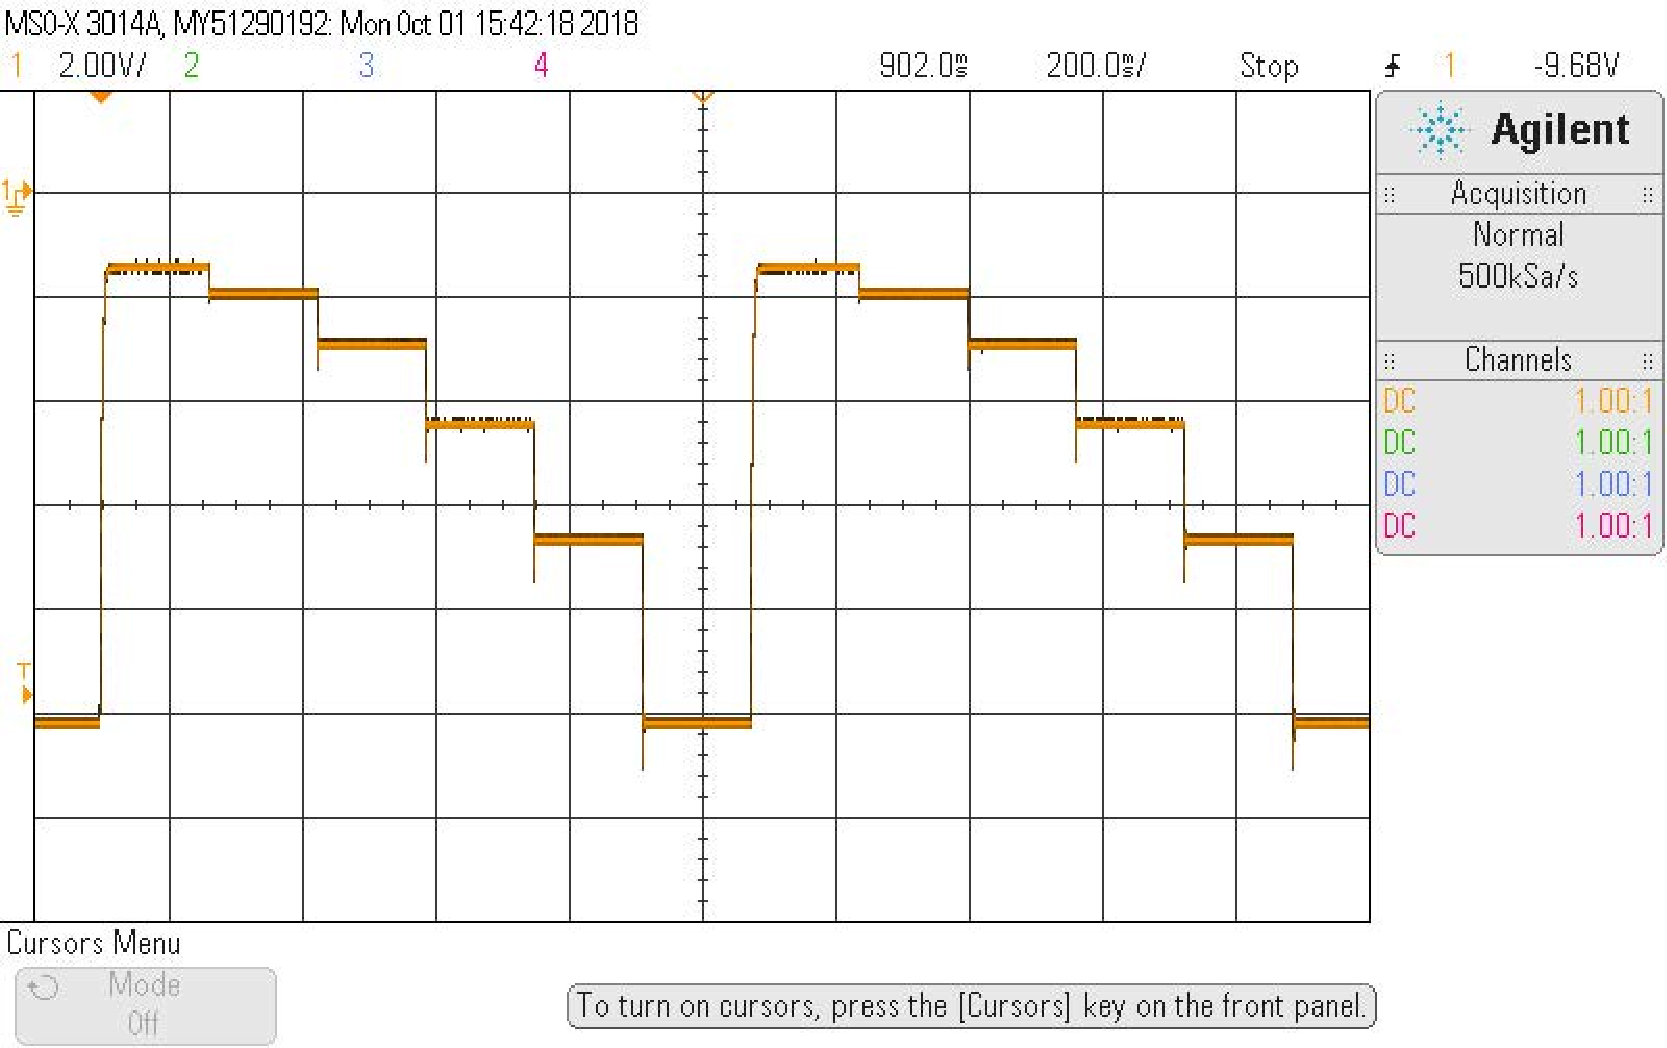
\includegraphics[height = 0.35\textheight]{converter_openloop.pdf}}
\caption{}
\label{fig:steps}
\end{figure}
Purpose of test: to compare hardware result Figure~\ref{fig:steps} with theoretical Figure~\ref{fig:out_parasitic}.
\begin{figure}[H]
\centering
\fbox{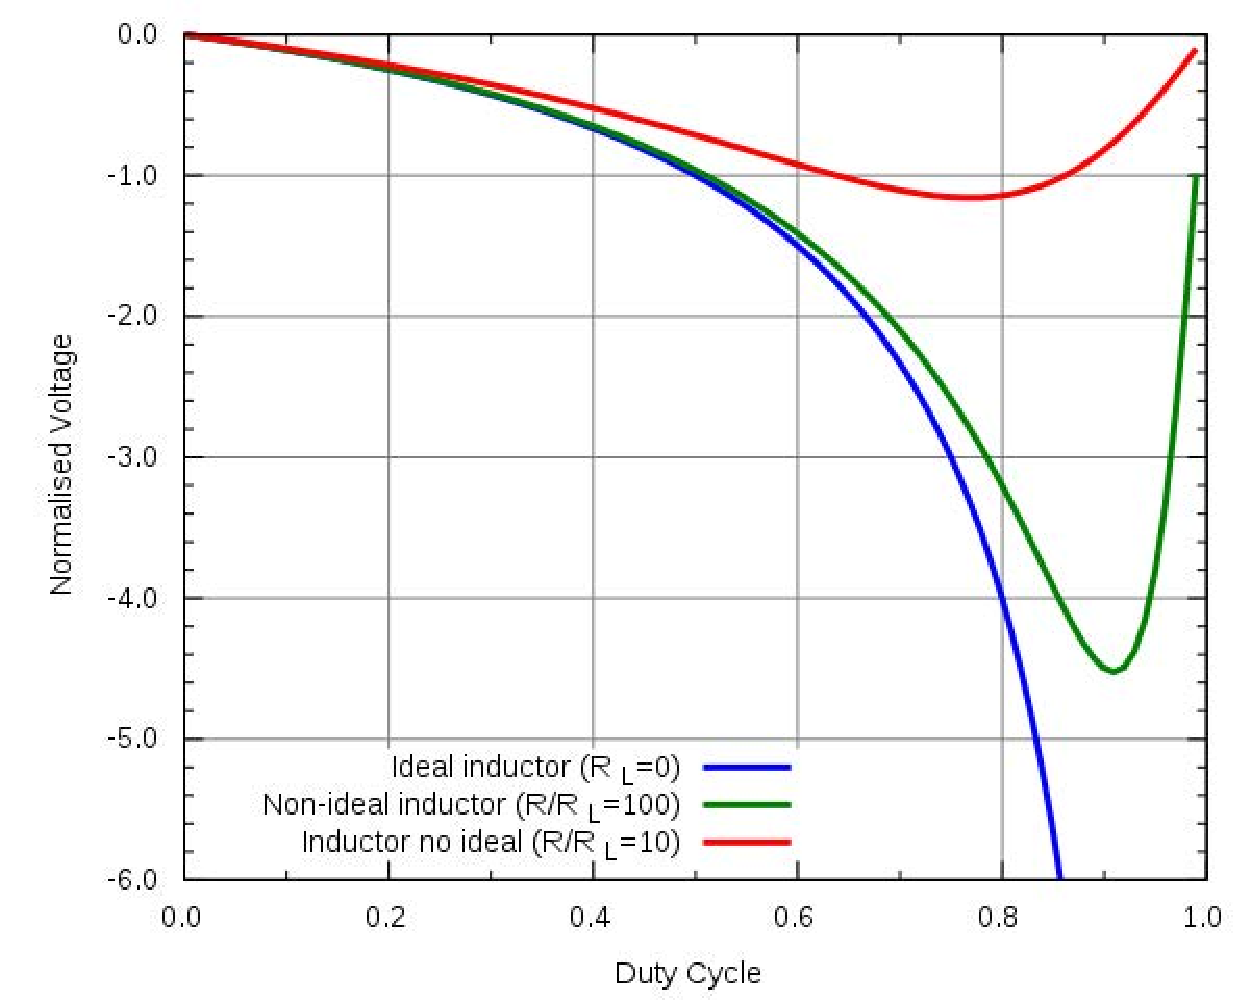
\includegraphics[height = 0.35\textheight]{tfout_parasitic.pdf}}
\caption{}
\label{fig:out_parasitic}
\end{figure}
%%%%%%%%%%%%%%%%%%%%%%%%%%%%%%%%%%%%%%%%%%%%%%%%%%%%%%%%%%%%%%%%%%%%%%%%%%%%%%%%
\subsubsection{Testing operating region limits}
A PWM signal of duty ratio $85 \ \mathsf{\%}$ was sent to the converter to test stability, safety, and power usage. A summary of the data produced in this experiment is provided in Table~\ref{tab:heating}.
\begin{table}[H]
    \centering
    \begin{tabular}{|c|c|c|}
    \hline
    Quantity & Value & Notes\\
    \hline
    $d$ & $85 \ \mathsf{\%}$ &\\
    \hline
    $v_o$ & $\minus 21 \ \mathsf{V}$ &\\
    \hline
    $v_g$ & $5 \ \mathsf{V}$ &\\
    \hline
    Output voltage ripple & $75 \ \mathsf{mV} \ (0.4 \ \mathsf{\%})$ &\\
    \hline
    Input current draw & $1.15 \ \mathsf{A}$&\\
    \hline
    \end{tabular}
    \caption{}
    \label{tab:heating}
\end{table}
Output voltage ripple here refers to the peak-to-peak MOSFET switching noise at this operating point. Converter voltage ripple $\approx (1/3) \times \text{ switching noise}$. At this operating point the $100 \ \mathsf{\Omega}$ resistor dissipated $\sim 4 \ \mathsf{W}$ of heat (and became far too hot to touch).
%%%%%%%%%%%%%%%%%%%%%%%%%%%%%%%%%%%%%%%%%%%%%%%%%%%%%%%%%%%%%%%%%%%%%%%%%%%%%%%%
%%%%%%%%%%%%%%%%%%%%%%%%%%%%%%%%%%%%%%%%%%%%%%%%%%%%%%%%%%%%%%%%%%%%%%%%%%%%%%%%
%%%%%%%%%%%%%%%%%%%%%%%%%%%%%%%%%%%%%%%%%%%%%%%%%%%%%%%%%%%%%%%%%%%%%%%%%%%%%%%%
\subsection{Controller}
% Collection of data to present performance of control regime in hardware is ongoing. Results are not in a state to present in this report at this time.
The performance of controller was tested on hardware. The reference points were hard-coded \{-1V, -11V, -6V, -1V, -8V, -11V \} with 200ms interval.The result is provided in Figure \ref{fig:performance}.

The controller was able to track the reference voltage well with \hl{little} overshoot and \hl{small} settling time. The summary of performance is provided in Table \ref{tab:performance}.

\begin{table}[h]
\centering
\begin{tabular}{|c|c|c|}
    \hline
    Quantity        & Value  & Notes \\ \hline \hline 
    Settling time   & 26.4ms &  Reference -1V to -8V\\ \hline
    Overshoot       & 2.4V   &  Reference -1V to -8V\\ \hline
    Output voltage ripple & 23.7mV (XXX \%) & Reference 2V\\
    \hline
\end{tabular}
\caption{Summary of controller performance}
\label{tab:performance}
\end{table}

The controller performned well, however when the reference changes from -1V to -11V, the saturation can be seen. This could be due to anti-windup. It was later discovered that reducing the gain of anti-windup resulted in less saturation and better performance. 
\begin{figure}[H]
    \begin{framed}
    \captionsetup[subfigure]{justification = centering}
    \centering
    \begin{subfigure}[b]{0.8\textwidth}
    \centering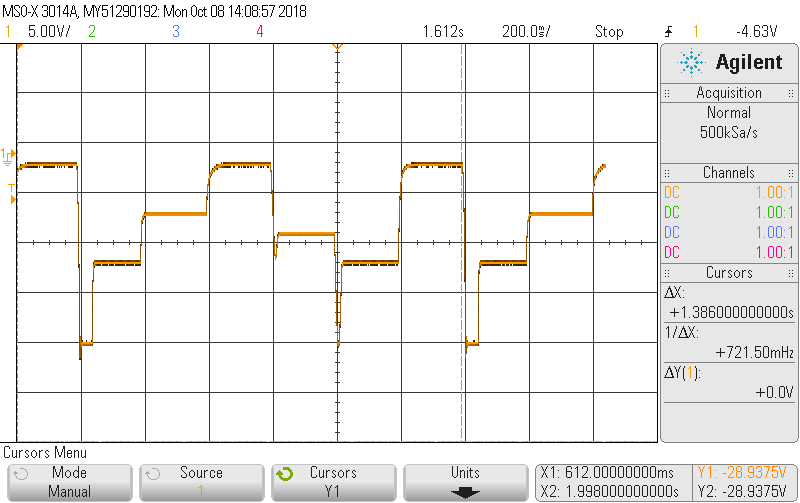
\includegraphics[width = \textwidth]{figures/result/changeRef.png}
    \caption{Output voltage response}
    % \label{fig:estimatingconditions1}
    \end{subfigure}
    \\[11pt]
    \begin{subfigure}[b]{0.45\textwidth}
    \centering
    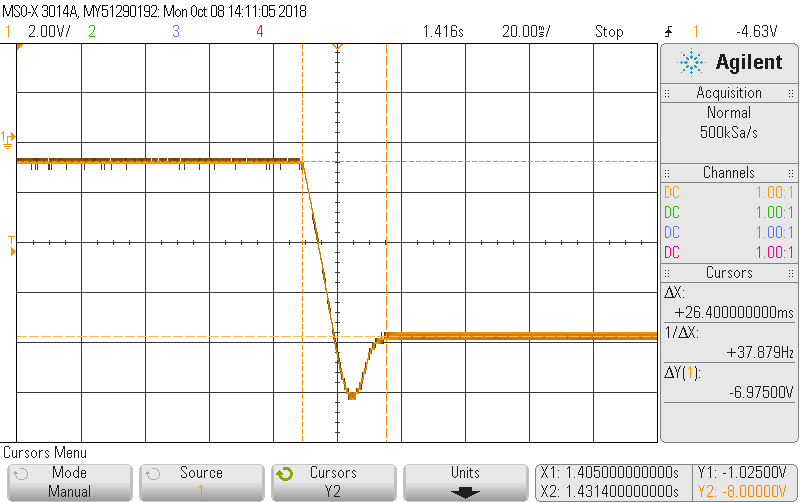
\includegraphics[width = \textwidth]{figures/result/overshoot1to8.png}
    \caption{Overshoot and settling time}
    % \label{fig:estimatingfirst}
    \end{subfigure}
    \hfill
    \begin{subfigure}[b]{0.45\textwidth}
    \centering
    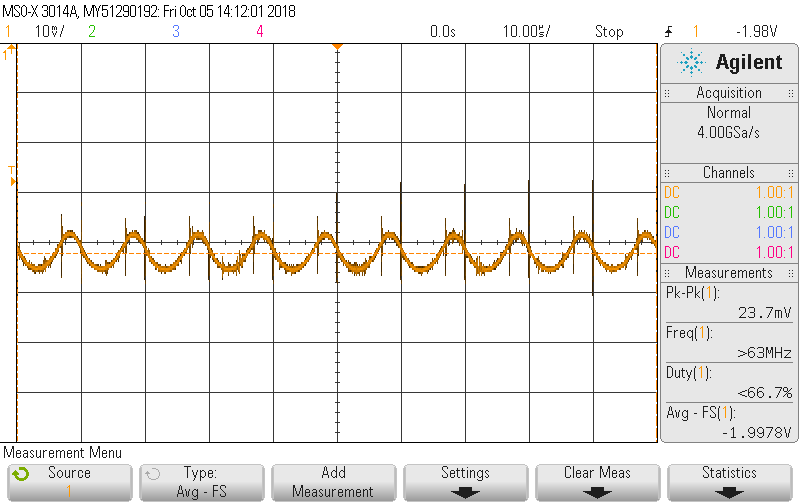
\includegraphics[width = \textwidth]{figures/result/ripple.png}
    \caption{Voltage ripples}
    % \label{}
    \end{subfigure}
    \end{framed}
    % \vspace*{-8mm}
    \caption{\hl{TODO}}
    \label{fig:performance}
\end{figure}

% \begin{figure}[h]
% \centering
% \begin{tabular}{cc}
%     \multicolumn{2}{c}{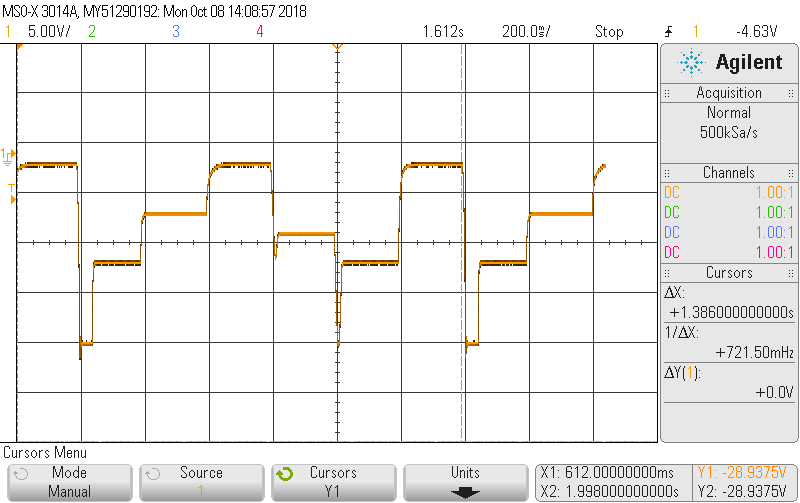
\includegraphics[width = 0.7\textwidth]{figures/result/changeRef.png}} \\
%     \multicolumn{2}{c}{(a) Output voltage response} \\ \\
%     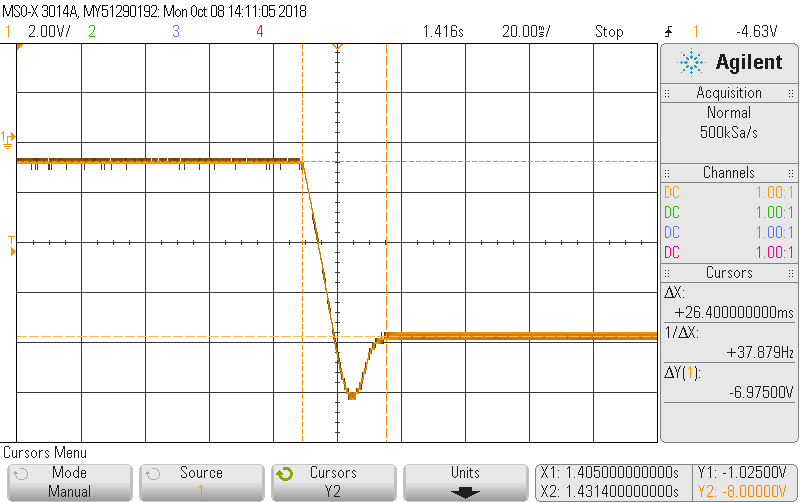
\includegraphics[width=.5\linewidth]{figures/result/overshoot1to8.png}
%     &
%     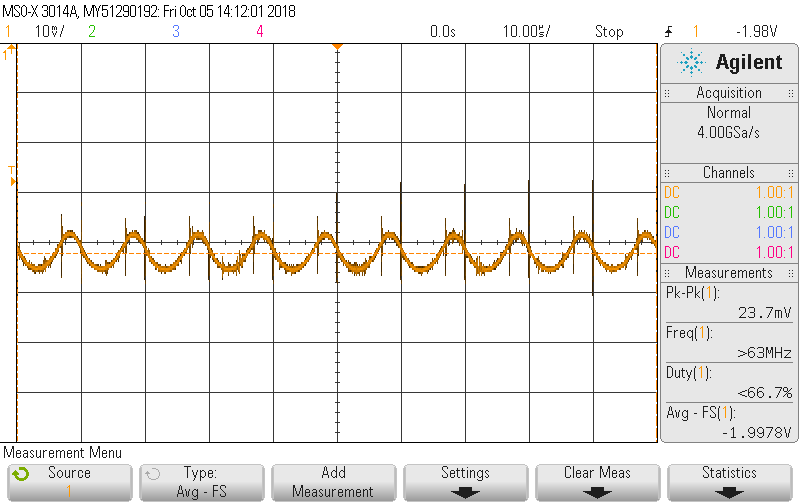
\includegraphics[width=.5\linewidth]{figures/result/ripple.png}\\
%     (b) Overshoot and settling time & (c) Voltage ripples     
% \end{tabular}
% \caption{Controller performance}
% \label{fig:performance}
% \end{figure}

\hl{Add function generator stuff here?}

%%%%%%%%%%%%%%%%%%%%%%%%%%%%%%%%%%%%%%%%%%%%%%%%%%%%%%%%%%%%%%%%%%%%%%%%%%%%%%%%
%%%%%%%%%%%%%%%%%%%%%%%%%%%%%%%%%%%%%%%%%%%%%%%%%%%%%%%%%%%%%%%%%%%%%%%%%%%%%%%%
%%%%%%%%%%%%%%%%%%%%%%%%%%%%%%%%%%%%%%%%%%%%%%%%%%%%%%%%%%%%%%%%%%%%%%%%%%%%%%%%